\subsection{Klassifikation (FU/DFG + IDS Grammatik)}

\begin{frame}
  {Ziele der Klassifikation}
  \begin{itemize}
    \item Entwicklung von in den Daten verankerten Klassifikationen
    \item Ausschlusskriterium: schlechte automatische Klassifizierbarkeit\\
      (\alert{nicht} so wie in Biber & Egbert 2016)
    \item Feststellen der Zusammensetzung von (Web-)Korpora,\\
      Vergleich z.\,B.\ DeReKo vs.\ DECOW
    \item Generierung von Metadaten\\
      inkl. \alert{Interpretation} für trad.\ Korpuslinguistik
    \item infragekommende Merkmale für datengetriebene Klassifikation:\\
      \alert{grammatische Merkmale} (COReX),\\
      \alert{lexikalische Verteilungen} (Topicmodelle, COReKO)
  \end{itemize}
\end{frame}

\begin{frame}
  {Verfahren bei COReKO}
  \begin{itemize}
    \item Klassifikation nach \alert{Themengebiet} (=Topikdomäne)
    \item ca.\ 20 Kategorien (Politik, Sport, Kunst, Alltag usw.)
    \item Goldstandards für DECOW und DeReKo
    \item erster Schritt: \alert{Topikmodellierung} (LSI, LDA)\\
      geneeriert Topik-Dokument-Matrizen (TDM)
    \item zweiter Schritt: \alert{überwachte Klassifikation}\\
      der Themengebiete mit TDM als Merkmale
  \end{itemize}
\end{frame}

\begin{frame}
  {Experiment COReKo 1}
  \begin{itemize}
    \item Goldstandard: ca.\ 800 Dokumente DECOW und 800 DeReKo
    \item Topicmodelling: GenSim (LSI. LDA)
    \item Topikdomänen-Klassifizierer: SVM
    \item verschiedene Vorverarbeitungsvarianten\\
      (meistens am besten: lemma+POS, nur Inhaltswörter)
    \item 20--90 Topiks
    \item inkrementelles Zumischen von Dokumenten zum Goldstandard zur Stabilisierung der Topiks (Entfernung für Klassifizierung der Topikdomänen)
  \end{itemize}
\end{frame}

\begin{frame}
  {Ergebnisse COReKo 1}
  Genauigkeit (10CV) nur DECOW\\
  \centering
  \vspace{0.5cm}
  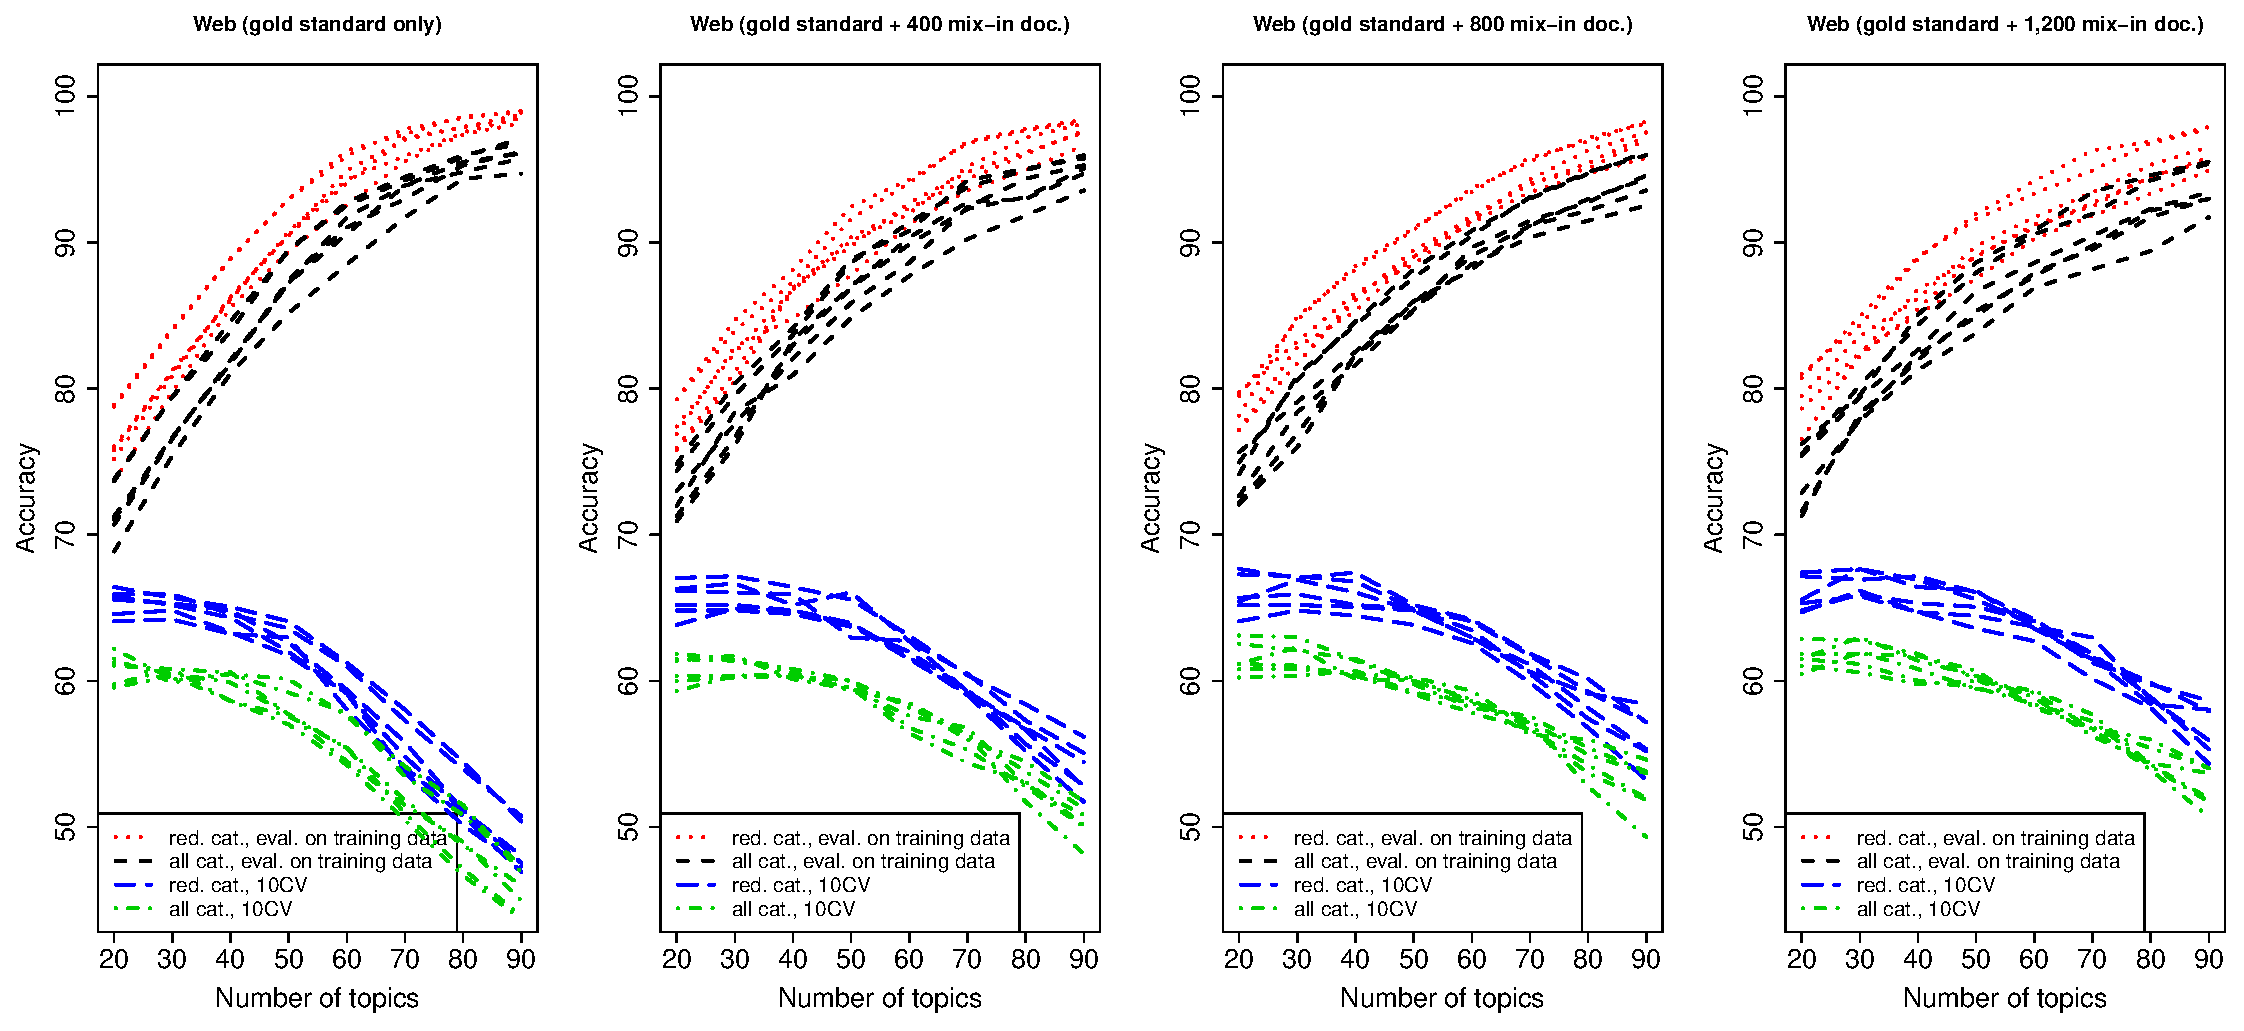
\includegraphics[width=0.8\textwidth]{graphics/cow}
\end{frame}

\begin{frame}
  {Ergebnisse COReKo 1}
  Genauigkeit (10CV) nur DeReKo\\
  \centering
  \vspace{0.5cm}
  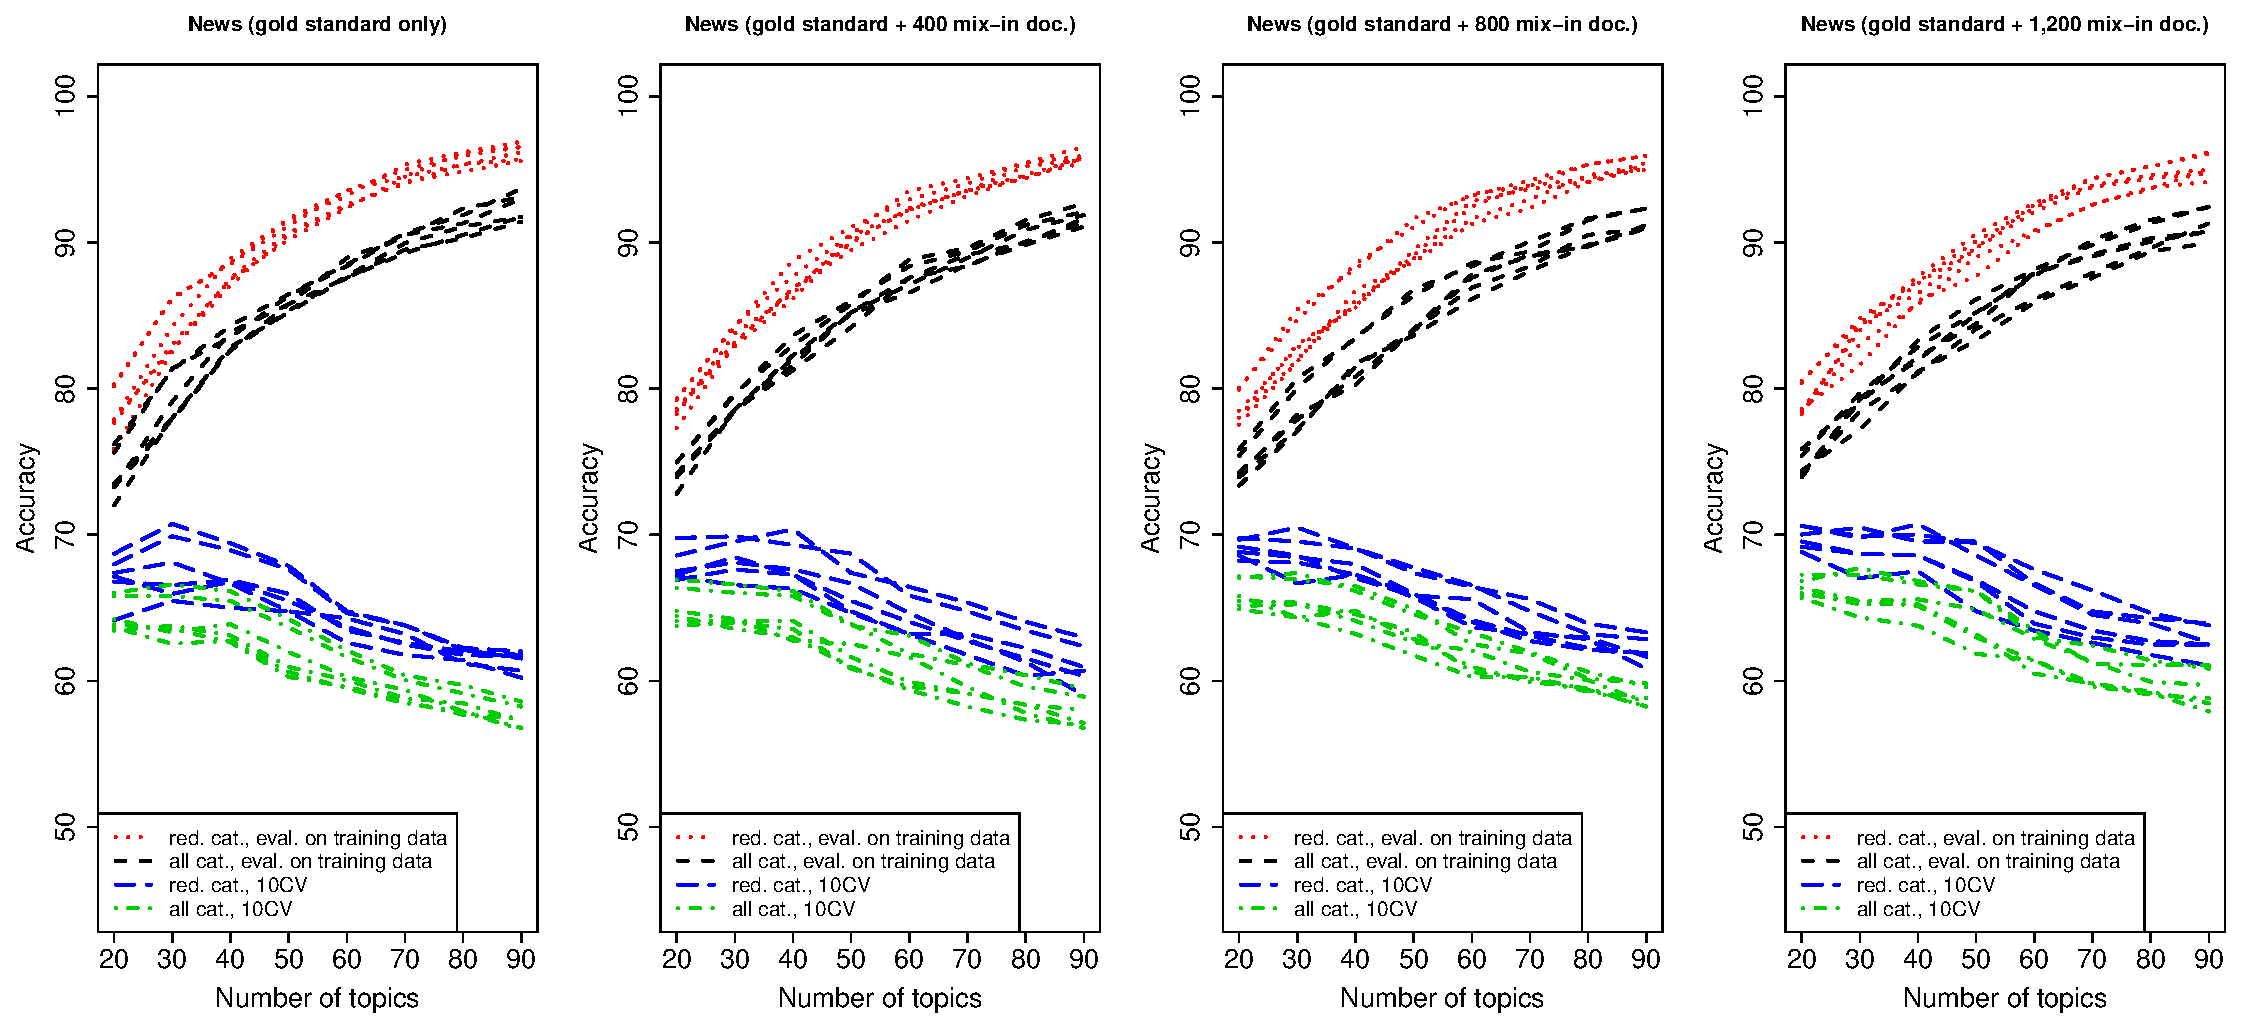
\includegraphics[width=0.8\textwidth]{graphics/dereko}
\end{frame}

\begin{frame}
  {Ergebnisse COReKo 1}
  Genauigkeit (10CV) vereinte Daten\\
  \centering
  \vspace{0.5cm}
  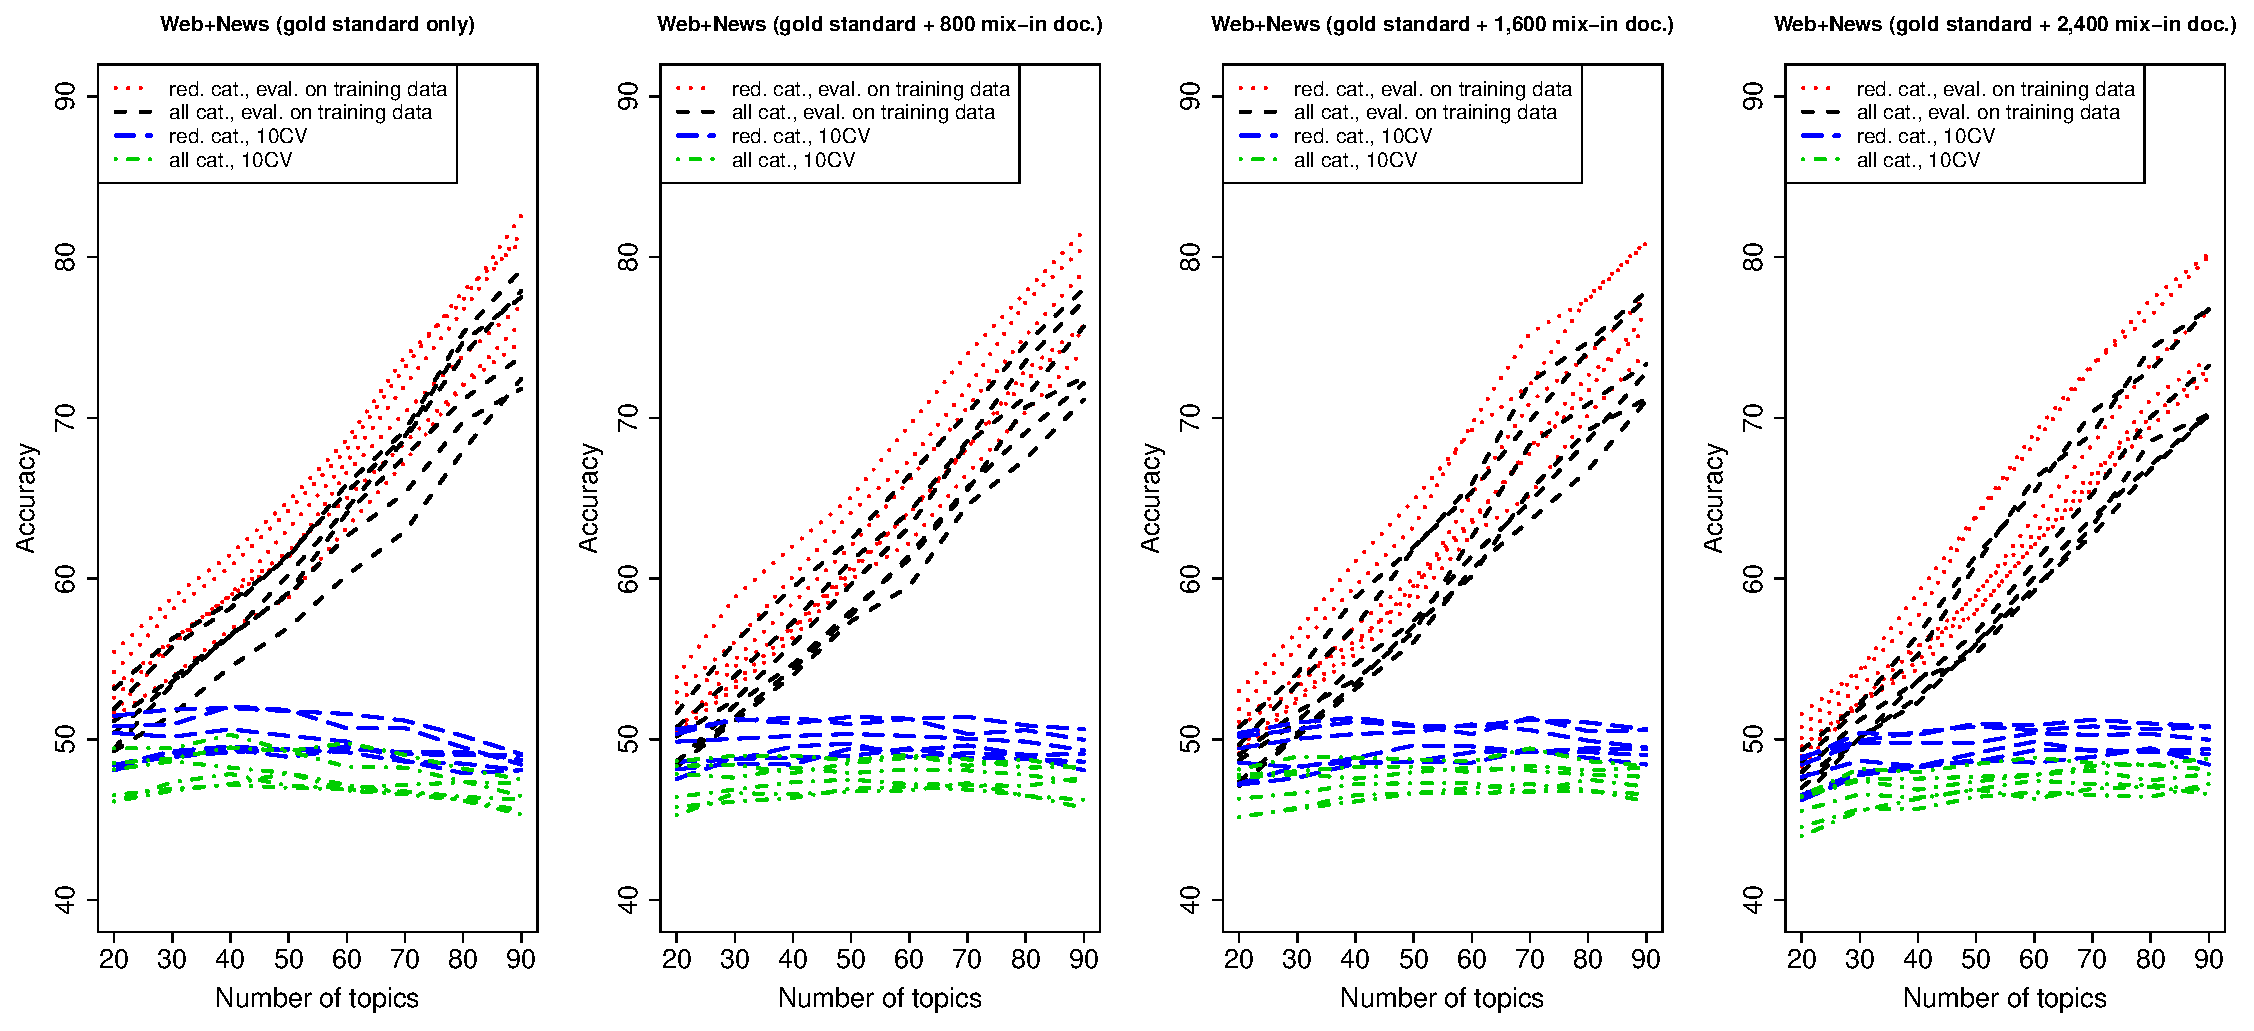
\includegraphics[width=0.8\textwidth]{graphics/coreko}
\end{frame}

\begin{frame}
  {Gründe für die mäßige Qualität}
  \centering
  \scalebox{0.55}{\begin{tabular}{|llcccccccc|}
    \hline
    %\multicolumn{2}{|c}{\textbf{COW}} & \multicolumn{8}{c|}{\textbf{Classified}} \\
    \multicolumn{2}{|c}{\textbf{Web}} & \multicolumn{8}{c|}{\textbf{Classified}} \\
     && \rot{\textbf{PolSoc~}} & \rot{\textbf{Busi}} & \rot{\textbf{Life}} & \rot{\textbf{Arts}} & \rot{\textbf{Public~}} & \rot{\textbf{Law}} & \rot{\textbf{Beliefs~}} & \rot{\textbf{Hist}} \\
   \hline
   \multirow{8}{*}{\rot{\textbf{Annotated}}} & \textbf{PolSoc}  & \textbf{26} &  12 &  10 &   1 &   1 &   0 &   1 &   0 \\ 
     & \textbf{Busi}    &  5 & \textbf{105} &  40 &   7 &   1 &   2 &   1 &   1 \\ 
     & \textbf{Life}    &  3 &  14 & \textbf{286} &   6 &   4 &   1 &   1 &   1 \\ 
     & \textbf{Arts}    &  3 &   2 &  36 &  \textbf{78} &   1 &   0 &   2 &   6 \\ 
     & \textbf{Public}  &  0 &   3 &  11 &   0 &   \textbf{9} &   1 &   0 &   0 \\ 
     & \textbf{Law}     &  3 &   9 &   8 &   0 &   1 &   \textbf{8} &   0 &   0 \\ 
     & \textbf{Beliefs} &  4 &   3 &  11 &   6 &   1 &   0 &  \textbf{30} &   1 \\ 
     & \textbf{Hist}    &  9 &   0 &   9 &   7 &   1 &   1 &   2 &  \textbf{15} \\ 
     \hline
   \end{tabular}}
\end{frame}
 
\begin{frame}
  {Gründe für die mäßige Qualität}
  \centering
 \scalebox{0.55}{\begin{tabular}{|llcccccc|}
    \hline
     %\multicolumn{2}{|c}{\textbf{DeReKo}} & \multicolumn{6}{c|}{\textbf{Classified}} \\
     \multicolumn{2}{|c}{\textbf{News}} & \multicolumn{6}{c|}{\textbf{Classified}} \\
     && \rot{\textbf{PolSoc~}} & \rot{\textbf{Busi}} & \rot{\textbf{Life}} & \rot{\textbf{Indiv}} & \rot{\textbf{Arts}} & \rot{\textbf{Public}} \\
    \hline
     \multirow{6}{*}{\rot{\textbf{Annotated}}}& \textbf{PolSoc}  & 223 & 6 & 39 &  0 &  0 &  8 \\
     & \textbf{Busi}    &  20 & 24 &   9 &  0 &  0 &  0 \\
     & \textbf{Life}    &  24 &  1 & 324 &  0 &  0 &  1 \\
     & \textbf{Indiv}   &   5 &  0 &  17 &  0 &  0 &  1 \\
     & \textbf{Arts}    &   2 &  0 &  28 &  0 &  6 &  0 \\
     & \textbf{Public}  &  35 &  0 &  30 &  0 &  0 & 34 \\
    \hline
  \end{tabular}}
\end{frame}
 
\begin{frame}
  {Gründe für die mäßige Qualität}
  \centering
\scalebox{0.55}{\begin{tabular}{|llccccccccc|}
    \hline
     \multicolumn{2}{|c}{\textbf{Pooled}} & \multicolumn{9}{c|}{\textbf{Classified}} \\
     && \rot{\textbf{PolSoc~}} & \rot{\textbf{Busi}} & \rot{\textbf{Med~}} & \rot{\textbf{Life}} & \rot{\textbf{Arts}} & \rot{\textbf{Public~}} & \rot{\textbf{Law}} & \rot{\textbf{Beliefs~}} & \rot{\textbf{Hist}} \\
    \hline
    \multirow{9}{*}{\rot{\textbf{Annotated}}} & \textbf{PolSoc}   & \textbf{199} &   7 &   0 & 109 &   0 &  12 &   0 &   0 &   0 \\ 
    & \textbf{Busi}     &  18 &  \textbf{23} &   0 & 172 &   0 &   2 &   0 &   0 &   0 \\ 
    & \textbf{Med}  &   6 &   0 &   \textbf{0} &  29 &   0 &   1 &   0 &   0 &   0 \\ 
    & \textbf{Life}     &  25 &   4 &   0 & \textbf{632} &   0 &   5 &   0 &   0 &   0 \\ 
    & \textbf{Arts}     &   2 &   2 &   0 & 160 &   \textbf{0} &   0 &   0 &   0 &   0 \\ 
    & \textbf{Public}   &  46 &   2 &   0 &  56 &   0 &  \textbf{19} &   0 &   0 &   0 \\ 
    & \textbf{Law}      &   8 &   0 &   0 &  31 &   0 &   0 &   \textbf{0} &   0 &   0 \\ 
    & \textbf{Beliefs}  &   0 &   0 &   0 &  59 &   0 &   0 &   0 &   \textbf{0} &   0 \\ 
    & \textbf{Hist}     &   4 &   0 &   0 &  50 &   0 &   0 &   0 &   0 &   \textbf{0} \\ 
    \hline
 \end{tabular}}
\end{frame}

\begin{frame}
  {Schlussfolgerungen}
  \begin{itemize}
    \item größere Goldstandard-Datensätze
    \item verändertes Klassifikationsschema
    \item auch Verfügbarmachen der induzierten Topik-Distribution\\
      als Metadaten 
  \end{itemize}
\end{frame}
